\chapter{Capital Buffers, Cash Motion, and the Business of Keeping One's Word}

This chapter treats the Wall Street interviews as a field lecture on wealth. The material does not come to us as a polished board derivation. It comes in bursts: a repeated question about having been broke, a claim of forty-nine years in business, a claimed \$400 million revenue year, a trader moving half a billion dollars a day, and then a sequence of compressed rules about survival, discipline, circulation, and judgment. If we keep the lecture in its spoken order, the underlying structure becomes clear. Wealth is not presented as a mystical quality. It is presented as buffer, motion, recovery, reputation, and selection.

\section{Teaser, Scale, and the Governing Question}

The lecture opens by throwing scale at us before it gives us theory. One person says he has been broke multiple times. Another says he has been an entrepreneur for forty-nine years. A construction business is said to have done roughly \$400 million in a single year. A financier says he sits on five boards, runs seven companies, and trades half a billion dollars of stock in a day. We may record the scale claims succinctly as
\begin{align}
t_{\text{entrepreneur}} &\approx 49\,\text{yr},\\
Y_{\max} &\approx 4.0\times 10^8\,\text{USD}\,\text{yr}^{-1},\\
V_{\text{trade}} &\approx 5.0\times 10^8\,\text{USD}\,\text{day}^{-1},\\
N_{\text{boards}} &= 5,\qquad N_{\text{companies}} = 7.
\end{align}
A further internet rumor of roughly \$1.8 billion in personal wealth is mentioned, though the speaker himself declines to certify it. We should therefore treat every such number as an interview claim, not as an independently verified datum.

The point of this opening is not numerical fetishism. The lecture is arranging the problem. We are shown that extreme scale and repeated failure can coexist, and we are then asked what law, if any, sits underneath that coexistence. The host makes the governing question explicit: what do wealthy operators know about money that most people do not? That question is the thread that ties the whole lecture together.

\section{Wall Street as a Field Study of Scarce Advice}

Before a serious answer appears, the lecture forces us through refusal. The host approaches people quickly, is waved off, negotiates for thirty seconds, cites past interviews, and keeps moving. This sequence is part of the pedagogy. Advice does not arrive in seminar conditions. It arrives under scarcity, impatience, and social friction.

The first respondent who eventually yields more than a brush-off gives a preliminary answer: work hard; the rest is overrated. That line is not dismissed, but the lecture does not stop there. It keeps walking with the man. This is important for the rhythm of the notes. The talk is not content with a slogan. It keeps pressing until a mechanism appears. We should preserve that pressure on the page.

\section{Capital Buffer and Business Survival}

Once the conversation lengthens, the first hard mechanism appears immediately. The host frames the problem by invoking the common claim that many businesses do not make it past five years. The reply is laconic and structural: they are underfinanced.

\subsection{Question \& Answer}

\paragraph{Question.} What is the most common mistake that destroys a business before it has had time to mature?

\paragraph{Answer.} The speaker's answer is not poor branding, insufficient passion, or lack of ambition. It is simply this: the business is underfinanced.

We may encode the host's framing by the rough empirical statement
\begin{equation}
p_{\text{business fail by 5y}} \approx 0.8.
\end{equation}
The exact number is not the point. The point is that the answer lands at the level of capital structure.

\begin{definition}
We call \(K_{\text{buffer}}\) the liquid capital available to carry a firm through ordinary operating burn and through the shocks that are not optional but only uncertain in timing and magnitude.
\end{definition}

Now let us write the speaker's verbal rule in a form that can be used. Let \(B\) denote the ordinary burn per unit time, \(T\) the horizon over which the firm must survive, and \(S\) the reserve required for overruns, delays, or other disturbances. Then the lecture's survival law is the inequality
\begin{equation}
K_{\text{buffer}} \ge BT + S.
\end{equation}

\begin{proposition}[Buffer condition]
A business becomes structurally fragile when its available liquidity falls below the sum of ordinary carrying cost and shock reserve.
\end{proposition}

\begin{proof}
The ordinary cost of staying alive over horizon \(T\) is \(BT\). But the speaker's entire point is that life does not present a frictionless horizon; it presents bumps along the road. Those bumps require extra reserve \(S\). Hence the minimum protected position is \(BT+S\). If \(K_{\text{buffer}}<BT+S\), then the business may survive only by luck rather than by financial preparation.
\end{proof}

A useful limiting case makes the point sharper. If
\begin{equation}
K_{\text{buffer}} = BT,
\end{equation}
then the firm has financed ordinary survival and nothing more. In that case, any nonzero shock \(S>0\) is enough to expose the weakness. This is precisely why the interviewee adds that luck is real, but the safest way is to be well financed.

The lecture immediately places this financial mechanism beside a social one. The same speaker says he did not come from money, that his parents were not wealthy, and that the desire was to create success for himself. The notes should keep both levels in view. Desire provides direction; capital provides endurance. The lecture's order matters here. Ambition is not denied, but it is made answerable to a runway condition.

That same interview then folds sales back into the argument. In a competitive field such as construction, the speaker says, one sells by doing the right job. The work product is the best three-dimensional business card one can have. The connection is exact. The buffer keeps the firm alive long enough to produce the work; the work, if it is sound, markets the firm better than any pitch.

\section{Honor, Clients, Family, and the Outside Option}

The lecture does not leave the construction interview at the level of finance. It widens almost immediately into operating constraints. The speaker says: be honest, keep the clients satisfied, put your family first. He adds that faith has been at the top of the list, and that early risk felt easier because there was not much to lose: if things failed, he could go back to his tools.

Here the host's own recap is important. He does not merely say that the interview was strong; he extracts a rule from it. If you do not keep your word in business, you have no business. That sentence is sufficiently central that it deserves a simple update law:
\begin{equation}
\mathcal{R}_{t+1} = \mathcal{R}_t + \alpha M_t - \beta D_t,
\end{equation}
where \(\mathcal{R}_t\) is the stock of reputation, \(M_t\) counts commitments met, and \(D_t\) counts commitments defaulted on or broken.

The lecture does not write that equation, but it clearly thinks in that direction. Trust is cumulative. So is distrust. Promises kept add to the usable stock of confidence; promises broken subtract from it, often with larger magnitude than the gains arrived by. The speaker's emphasis on client satisfaction therefore belongs not to moral ornament but to the mechanics of repeated business.

The remark about risk also has a precise place. Risk appetite is not treated as an abstract virtue. It depends on the outside option. If one can go back to a trade, risk looks different than it does to someone whose floor is much lower. The lecture is careful here: it neither glorifies recklessness nor denies the role of courage. It locates courage inside circumstances.

\section{Saving, Fear, Emotion, and Time Ownership}

The next Wall Street interview narrows the frame from firm survival to personal financial conduct. The advice comes rapidly and in short strokes: save every penny you can; when you are young you think money grows on trees; fear of failure is a powerful motivator; do not invest with friends or family; billionaires take emotion out of money; communication matters; speak the truth; if you do not keep your word, you will not last.

Several further details should remain visible because they give the advice its social texture. The speaker says he became a millionaire at roughly thirty-five. He tells younger people to work hard at school, to expect a long slog, and to think in five- and ten-year plans. The host then synthesizes the lesson into a sharper entrepreneurial claim: if your goal is financial freedom, do not imagine that dependence on another person's paycheck automatically gets you there. Buy back your time. Delegate.

The lecture is therefore not teaching thrift in isolation. It is teaching thrift as preparation for autonomy. Savings are not yet wealth in the full sense. They are accumulated optionality.

\section{Motion, Loss, and Exchange}

The next interview introduces the lecture's central tension. Here the speaker insists that money has to keep moving. In order for it to grow and in order for it to work for you, it cannot simply lie idle in a bank or under a mattress. The lecture has now placed two imperatives side by side: save every penny, and keep money moving.

\subsection{Question \& Answer}

\paragraph{Question.} Must wealth be preserved by saving, or increased by circulation? Are the two instructions contradictory?

\paragraph{Answer.} They are contradictory only if we force one variable to play two different roles. The lecture becomes coherent as soon as we distinguish reserve from deployment.

Let \(W_t\) denote wealth or usable capital at time \(t\), let \(s_t\) denote fresh saving, let \(I_t\) denote deployed capital, let \(r_t\) denote the return on deployed capital, and let \(L_t\) denote losses. Then a minimal update law is
\begin{equation}
W_{t+1} = W_t + s_t + r_t I_t - L_t.
\end{equation}
In this form the two imperatives no longer conflict. Saving is capital formation. Motion is productive deployment.

If one refuses deployment altogether, so that \(I_t=0\), then the rule reduces to
\begin{equation}
W_{t+1} = W_t + s_t - L_t.
\end{equation}
This may be safe relative to reckless speculation, but it does not compound through return. On the other hand, if one deploys aggressively without maintaining reserve, then growth becomes fragile. The lecture's real answer is therefore a two-layer rule: keep enough liquidity to survive; move enough capital to grow.

\begin{figure}
\centering
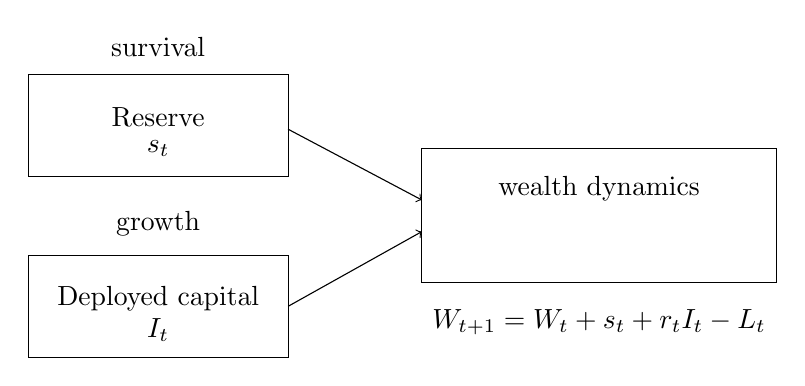
\begin{tikzpicture}[x=1cm,y=1cm]
\draw (0,0.4) rectangle (3.3,1.7);
\node at (1.65,1.15) {Reserve};
\node at (1.65,0.75) {\(s_t\)};
\node at (1.65,2.05) {survival};

\draw (0,-1.9) rectangle (3.3,-0.6);
\node at (1.65,-1.15) {Deployed capital};
\node at (1.65,-1.55) {\(I_t\)};
\node at (1.65,-0.2) {growth};

\draw (5.0,-0.95) rectangle (9.5,0.75);
\node at (7.25,0.25) {wealth dynamics};
\node at (7.25,-1.45) {\(W_{t+1}=W_t+s_t+r_t I_t-L_t\)};

\draw[->] (3.3,1.0) -- (5.0,0.10);
\draw[->] (3.3,-1.25) -- (5.0,-0.30);
\end{tikzpicture}
\caption{Editorial reconstruction of the lecture's two-layer capital logic: reserve supports endurance, deployment supports growth. The lecture gives the distinction verbally rather than diagrammatically, but the separation is essential to its argument.}
\end{figure}

Once this is in place, the interview turns sharply toward loss. The speaker says his worst financial decision was marriage, more precisely a divorce that wiped him out. Whatever we make of the formulation, the lecture uses it to introduce a deeper point: what matters is not only loss, but recovery time.

Schematically,
\begin{equation}
T_{\text{rec}} \approx \frac{L}{\dot W_{\text{rebuild}}},
\end{equation}
where \(L\) is the effective loss and \(\dot W_{\text{rebuild}}\) is the rate at which one can rebuild wealth, capacity, or position. The transcript becomes unreliable when the speaker tries to turn this into an age-specific numerical example, but the stable content is clear. The same loss is less punishing when there is more time, more energy, or more earning runway left with which to recover.

The lecture then rises from recovery to social selection. You are, the speaker says, the sum total of the people you spend time with. One must therefore distinguish socializing from networking. The crucial question is not whether one is in motion, but whether the motion contains an exchange. What is being bartered here?

\begin{definition}
For an interaction between parties \(i\) and \(j\), define the exchange value
\begin{equation}
E_{ij}=G_{ij}-C_{ij},
\end{equation}
where \(G_{ij}\) denotes gain and \(C_{ij}\) denotes cost, broadly construed to include information, opportunity, time, distraction, trust, and money.
\end{definition}

Then the lecture's language of assets and liabilities becomes
\begin{equation}
E_{ij}>0 \Rightarrow \text{asset-like relation}, \qquad
E_{ij}<0 \Rightarrow \text{liability-like relation}.
\end{equation}

From here comes the strangest and, in its own way, most memorable analogy in the lecture. The speaker turns to breathing: inhale, exhale. The body takes in oxygen and gives out carbon dioxide; the environment reverses the transaction. He then says contract, expand; contract, expand. We should not mistake this for literal science on the page. It is a metaphor for stable exchange. Pure intake suffocates the system; pure output empties it. A viable relation alternates.

\begin{remark}
The inhale--exhale language should be preserved as metaphor, not elevated into a physical theorem. Its function in the lecture is to move from money to reciprocity: every durable relation, commercial or personal, must be tested by the quality of its exchange.
\end{remark}

The interview concludes with the Einstein line that reality is merely an illusion, albeit a very persistent one. In the logic of this lecture, that remark serves as distance. Wealth, failure, and status all feel absolute when they are close. The speaker is trying to recover judgment by stepping back from the immediacy of appearances.

\section{Screening Ideas, Trades, and the Meaning of Rich}

There is a brief interruption in the flow for channel promotion, and then the lecture restarts in a cleaner register with a self-styled Einstein of Wall Street. The tone is lighter at first, even comic, but it quickly becomes systematic. The speaker again establishes scale and energy: age is not the main point, he says; the point is what one does with the day. Then the argument turns toward business screening.

The warning is that people fall in love with an idea without asking whether the idea can support a real business. The language given is a four-part screen: people, process, product, and profits. We may gather that into the tuple
\begin{equation}
\mathcal{S}(b)=\bigl(People(b),\,Process(b),\,Product(b),\,\Pi(b)\bigr),
\end{equation}
where \(\Pi(b)\) denotes the profitability of business \(b\).

The lecture is careful about the use of this screen. It is not merely a checklist. It is a discipline of detachment. If the idea cannot be profitable, cannot sustain a process, or cannot serve as the basis of an organization larger than the founder's self-image, then emotional attachment is not evidence in its favor. The same principle is then carried into trading: people fall in love with trades, become attached to ego, and lose the capacity to take gains or losses cleanly.

At this point the lecture also returns to the question of what it means to be rich. The speaker refuses to equate richness with the largest pile of money. He says, in effect, that family, meaningful work, and the ability to motivate and empower others count decisively. Yet the lecture does not become anti-monetary. It adds a boundary condition that deserves to remain in the notes: cash equals freedom; it does not equal happiness. One needs money. One simply must not confuse it with the whole end of life.

The final move is pedagogically elegant. How should a younger person choose an industry? The answer is observational rather than abstract. Walk around the school. Look at the phones, the computers, the shoes, the brands, the platforms, the loyalties. The lecture ends not with a hidden formula but with an instruction in seeing. We are to read consumption patterns as signals of where process, product, and profitability may already be aligned.

\section{Summary}

The lecture begins with numbers and ends with discrimination. In between, it gives us a chain of mechanisms. Businesses fail when they are underbuffered. Reputation compounds when commitments are met and decays when they are broken. Savings matter, but only as one layer of a larger capital logic; money must also be deployed if it is to work. Loss is governed not merely by size but by recovery time. Relationships, like trades, should be judged by the quality of the exchange they contain. And profits, though necessary, do not exhaust the meaning of being rich.

If we preserve the order in which the lecture unfolds, its structure becomes surprisingly strict. First we establish scale. Then we pay the price of obtaining advice. Then we get the first law of endurance. Then we widen from capital to character. Then we distinguish reserve from deployment. Then we move from motion to loss, from loss to recovery, and from recovery to exchange. Finally we return to business judgment in a more explicit language: people, process, product, profits. That is the spine of the chapter, and it is the reason the lecture feels more like a compact theory than a mere collage of street interviews.